\documentclass[12pt,a4paper]{article}
\usepackage{ctex}
\usepackage{amsmath,amscd,amsbsy,amssymb,latexsym,url,bm,amsthm}
\usepackage{epsfig,graphicx,subfigure}
\usepackage{enumitem,balance}
\usepackage{wrapfig}
\usepackage{mathrsfs,euscript}
\usepackage[usenames]{xcolor}
\usepackage{hyperref}
\usepackage[vlined,ruled,linesnumbered]{algorithm2e}
\hypersetup{colorlinks=true,linkcolor=black}

\newtheorem{theorem}{Theorem}
\newtheorem{lemma}[theorem]{Lemma}
\newtheorem{proposition}[theorem]{Proposition}
\newtheorem{corollary}[theorem]{Corollary}
\newtheorem{exercise}{Exercise}
\newtheorem*{solution}{Solution}
\newtheorem{definition}{Definition}
\theoremstyle{definition}

\renewcommand{\thefootnote}{\fnsymbol{footnote}}

\newcommand{\postscript}[2]
 {\setlength{\epsfxsize}{#2\hsize}
  \centerline{\epsfbox{#1}}}

\renewcommand{\baselinestretch}{1.0}

\setlength{\oddsidemargin}{-0.365in}
\setlength{\evensidemargin}{-0.365in}
\setlength{\topmargin}{-0.3in}
\setlength{\headheight}{0in}
\setlength{\headsep}{0in}
\setlength{\textheight}{10.1in}
\setlength{\textwidth}{7in}
\makeatletter \renewenvironment{proof}[1][Proof] {\par\pushQED{\qed}\normalfont\topsep6\p@\@plus6\p@\relax\trivlist\item[\hskip\labelsep\bfseries#1\@addpunct{.}]\ignorespaces}{\popQED\endtrivlist\@endpefalse} \makeatother
\makeatletter
\renewenvironment{solution}[1][Solution] {\par\pushQED{\qed}\normalfont\topsep6\p@\@plus6\p@\relax\trivlist\item[\hskip\labelsep\bfseries#1\@addpunct{.}]\ignorespaces}{\popQED\endtrivlist\@endpefalse} \makeatother

\begin{document}
\noindent

%========================================================================
\noindent\framebox[\linewidth]{\shortstack[c]{
\Large{\textbf{Lab00-Proof}}\vspace{1mm}\\
CS214-Algorithm and Complexity, Xiaofeng Gao, Spring 2020.}}
\begin{center}
\footnotesize{\color{red}$*$ If there is any problem, please contact TA Yiming Liu.}

% Please write down your name, student id and email.
\footnotesize{\color{blue}$*$ Name:Hongjie Fang  \quad Student ID:518030910150 \quad Email: galaxies@sjtu.edu.cn}
\end{center}

\begin{enumerate}
    \item
    Prove that for any integer $n>2$, there is a prime $p$ satisfying $n<p<n!$. {\color{blue}(Hint: consider a prime factor $p$ of $n!-1$ and prove by contradiction)}
    \begin{proof}
        Assume there exists an integer $n_0$ satisfying that there is no prime number in the interval $(n_0, n_0!)$. It is obvious that $(n_0! - 1, n_0!) = 1$ where $(x, y)$ denotes the greatest common divisor between $x$ and $y$. According to the definition of factorial, all the integers in range $[2, n_0]$ are divisors of $n_0!$. Owing to the obvious fact that $n_0! - 1$ and $n_0!$ do not have any common divisor except $1$, all the integers in range $[2, n_0]$ are not divisors of $(n_0!-1)$. Furthermore, $(n_0!-1)$ is not a prime number because it is in the interval $(n_0, n_0!)$, so $(n_0!-1)$ must have a prime factor $p$. Because all the integers in range $[2, n_0]$ is not a divisor of $(n_0!-1)$, then the prime factor $p$ must be strictly greater than $n_0$. Based on the statement above, we can draw a conclusion that there exists a prime factor $p$ of $(n_0!-1)$ satisfying $p \in (n_0, n_0!-1) \subseteq (n_0, n_0!)$, which contradicts the assumption that there is no prime number in the interval $(n_0, n_0!)$
    \end{proof}

    \item
    Use the minimal counterexample principle to prove that for any integer $n>17$, there exist integers $i_n\ge 0$ and $j_n\ge 0$, such that $n = i_n \times 4 + j_n \times 7$.
    \begin{proof}
        We define $P(n)$ as the statement that there exist integers $i_n\ge 0$ and $j_n\ge 0$, such that $n = i_n \times 4 + j_n \times 7$. If $P(n)$ is not always true for $n > 17$, then there are values of $n$ for which $P(n)$ is false, and there must be a smallest such value, say $n = k$.

        Since $4 \times 1 + 7 \times 2 = 18$, $4 \times 3 + 7 \times 1 = 19$ and $4 \times 5 + 7 \times 0 = 20$, we have $P(18)$, $P(19)$ and $P(20)$ are true and $k - 3 > 17$.

        Since $k$ is the smallest value for which $P(k)$ false, $P(k-1)$ true. Thus $P(k-3)$ is true, that is, $\exists i_{k-3} \ge 0$ and $j_{k-3} \ge 0$, such that $k - 3 = i_{k-3} \times 4 + j_{k-1} \times 7$.

        \begin{itemize}
            \item If $i_{k-3} > 0$, then there exist $i_k = i_{k-3} - 1 \geq 0, j_k = j_{k-3} + 1 \geq 0$,
            \begin{displaymath}
                k = i_{k-3} \times 4 + j_{k-3} \times 7 + 3 = (i_{k-3} - 1) \times 4 + (j_{k-3} + 1) \times 7 = i_k \times 4 + j_k \times 7
            \end{displaymath}
            \item If $i_{k-3} = 0$, then $7 | (k - 3)$. Owing to $k - 3 > 17$ we have $j_{k-3} \ge 3$. Thus there exist $i_k = 6 \ge 0, j_k = j_{k-3}-3 \ge 0$,
            \begin{displaymath}
                k = j_{k-3} \times 7 + 3 = 6 \times 4 + (j_{k-3} - 3) \times 7 = i_k \times 4 + j_k \times 7
            \end{displaymath}
        \end{itemize}

        In conclusion, there exist $i_k \ge 0$ and $j_k \ge 0$ that $k = i_k \times 4 + j_k \times 7$. We have derived a contradiction, which allows us to conclude that our original assumption is false, which means $P(n)$ is true for $n > 17$.
    \end{proof}

    \item
    Let $P=\{p_1, p_2, \cdots\}$ the set of all primes. Suppose that $\{p_i\}$ is monotonically increasing, i.e., $p_1=2$, $p_2=3$, $p_3=5$, $\cdots$. Please prove: $p_n<2^{2^n}$. {\color{blue}(Hint: $p_i \nmid (1+\prod_{j=1}^n p_j), i=1,2,\cdots,n$.)}
    \begin{proof}
        The $i$-th number in the sequence $\{p_i\}$ denotes the $i$-th smallest prime number. Let $P(n)$ be the statement that $p_n < 2^{2^n}$. We prove $P(n)$ is true for every $n \in \mathbb{N}_+$ by induction.

        \textbf{\color{blue}Basis Step}. $P(1)$ is true, since $p_1 = 2 < 4 = 2^{2^1}$.

        \textbf{\color{blue}Induction Hypothesis} For $k \geq 1$ and $1 \leq n \leq k$, $P(n)$ is true.

        \textbf{\color{blue}Proof of Induction Step}. Let us prove $P(k+1)$. According to the definition of prime number, it cannot be formed by multiplying two smaller number. So if a number greater than $1$ does not have any smaller prime divisor, it is bound to be a prime number. Notice that $p_{k+1} \leq \prod_{i=1}^k p_i + 1 \stackrel{\Delta}{=} m$, because if $p_{k+1} \geq m$, then $m$ must be the $(k+1)$-th prime number, since $m$ does not have any smaller prime divisor, that is, $\forall 1 \leq i \leq k, p_i \nmid m$. And that is because $\forall 1 \leq i \leq k, p_i \mid (m - 1)$ and $(m - 1, m) = 1$ where $(x, y)$ denotes the greatest common divisor between $x$ and $y$. As a result,

        \begin{equation}\label{eq3-1}
            p_{k+1} \leq 1 + \prod_{i=1}^k p_i < 1 + \prod_{i=1}^k 2^{2^i} = 1 + 2 ^ {\sum_{i=1}^k 2^i} = 1 + 2^{2^{k+1} - 2} = 1 + \frac{1}{4} \cdot 2^{2^{k+1}} < 2^{2^{k+1}}
        \end{equation}

        According to Equation   \eqref{eq3-1}, we prove $P(k+1)$ is true.

        \textbf{\color{blue}Conclusion}. $P(n)$ is true for every $n \in \mathbb{N}_+$.
    \end{proof}

    \item
    Prove that a plane divided by $n$ lines can be colored with only $2$ colors, and the adjacent regions have different colors.
    \begin{proof}
        Let $Q(n)$ be the statement that a plane divided by $n$ lines can be colored with only $2$ colors, and the adjacent regions have different colors.

        Without loss of generality, we suppose the $2$ colors are black and white.

        To make the statement more explicit, we define requirement $R$ as the adjacent regions have different colors. We also define a mapping $f_n: P_n \rightarrow \{0, 1\}$ as the feasible plan of painting a plane divided by $n$ lines with only 2 colors and meeting the requirement $R$, where $P_n = \{p_1^n, p_2^n, ..., p_m^n\}$ is a set of regions after division by $n$ lines, $0$ means the region is painted white, and $1$ means the region is painted black.

        We prove $Q(n)$ is true for $n \in \mathbb{N}$ by induction.

        \textbf{\color{blue}Basis Step}. $Q(0)$ is the statement that a plane without any division can be painted to meet the requirement $R$. Under this circumstance, $P_0 = \{P\}$, where $P$ denotes the whole plane. It is obvious that $f_n(P) = 0$ is a feasible plan, so $Q(0)$ is true.

        \textbf{\color{blue}Induction Hypothesis}. Assume $Q(k)$ is true for some $k \geq 0$, that is, a plane divided by $k$ lines can be painted with only $2$ colors while meeting requirement $R$. So for every valid $P_k$, there exists a mapping $f_k: P_k \rightarrow \{0, 1\}$ denoting a feasible plan.

        \textbf{\color{blue}Proof of Induction Step}. Now let us prove that $Q(k+1)$ is true. Choose a line from total $(k+1)$ lines randomly, and name it line $l$. According to Induction Hypothesis, we are able to find out a mapping $f_k: P_k \rightarrow \{0, 1\}$ denoting a feasible plan of painting, when only consider the rest $k$ lines. Line $l$ divide the plane into two parts, and let us name them $p'_0$ and $p'_1$. It is obvious that $p'_0 \cap p'_1 = \varnothing$ and $p'_0 \cup p'_1 = P$ where $P$ stands for the whole plane. Thus, the set $P_{k+1}$ is:

        \begin{equation}\label{eq4-1}
            P_{k+1} = \{p \cap p'_0 | p \in P_k \} \cup \{p \cap p'_1 | p \in P_k \}
        \end{equation}

        We generate a mapping $f_{k+1}$ by the following formula.

        \begin{equation}\label{eq4-2}
        f_{k+1}(p \cap p'_0) = f_{k}(p), \quad f_{k+1}(p \cap p'_1) = 1 - f_{k}(p) \quad  (p \in P_k)
        \end{equation}

        According to Equation \eqref{eq4-1}, Equation \eqref{eq4-2} forms a valid mapping from $P_{k+1}$ to $\{0,1\}$, which also means that it is a painting plan. Now we proof that it meets requirement $R$.

        Consider each pair of adjacent regions $(p_i^{k+1}, p_j^{k+1}) (i \neq j)$.
        \begin{itemize}
        \item \textbf{Situation A}: As Figure \ref{picA} shows, if $p_i^{k+1}$ and $p_j^{k+1}$ are divided by the new line $l$, then $p_0^k \stackrel{\Delta}{=} p_i^{k+1} \cup p_j^{k+1} \in P_k$. Without loss of generality, we assume $p_i^{k+1} \subseteq p'_0$ and $p_j^{k+1} \subseteq p'_1$. According to the Equation \eqref{eq4-2},
                \begin{displaymath}
                f_{k+1}(p_i^{k+1}) = f_k(p_0^k) \neq 1 - f_k(p_0^k) = f_{k+1}(p_j^{k+1})
                \end{displaymath}
        \item \textbf{Situation B}: As Figure \ref{picB} shows, if $p_i^{k+1}$ and $p_j^{k+1}$ are divided by one of the rest $k$ lines, then the new line $l$ makes no difference to them and they are already adjacent, that is, either $p_i^{k+1}$ and $p_j^{k+1}$ are from the same region when considering only line $l$. Without loss of generality, we assume that $p_i^{k+1} \subseteq p'_0, p_j^{k+1} \subseteq p'_0$ and $p_{i'}^k \cap p'_0 = p_i^{k+1}, p_{j'}^k \cap p'_0 = p_j^{k+1}$ where $p_{i'}^k \in P_k, p_{j'}^k \in P_k$, so $p_{i'}^k$ and $p_{j'}^k$ are adjacent. According to the Equation \eqref{eq4-2} and the Induction Hypothesis,
            \begin{displaymath}
            f_{k+1}(p_i^{k+1}) = f_k(p_{i'}^k) \neq f_k(p_{j'}^k) = f_{k+1}(p_j^{k+1})
            \end{displaymath}
        \end{itemize}
        \begin{figure}[htbp]
          \centering
          \begin{minipage}[b]{0.4\linewidth}
          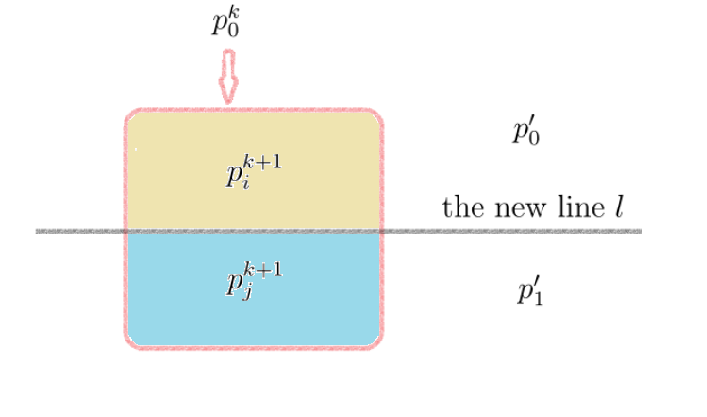
\includegraphics[width=3in]{pic1.png}
          \caption{Situation A}\label{picA}
          \end{minipage}
          \begin{minipage}[b]{0.4\linewidth}
          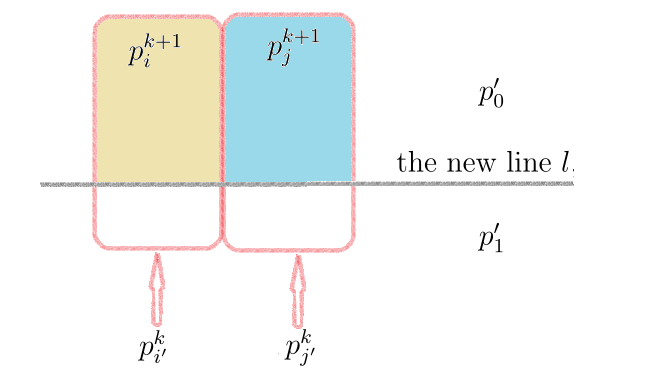
\includegraphics[width=3in]{pic2.png}
          \caption{Situation B}\label{picB}
          \end{minipage}
        \end{figure}

        In summary, for each pair of adjacent regions $(p_i^{k+1}, p_j^{k+1}) (i \neq j)$, we have $f_{k+1}(p_i^{k+1}) \ne f_{k+1}(p_j^{k+1})$. Thus, the mapping $f_{k+1}: P_{k+1} \rightarrow \{0, 1\}$ is a feasible plan of painting a plane divided by $(k+1)$ lines with only $2$ colors and meeting the requirement that the adjacent regions have different colors, that is, $Q(k+1)$ is true.

        \textbf{\color{blue}Conclusion}. $Q(n)$ is true for every $n \in \mathbb{N}$.
    \end{proof}

\end{enumerate}

\vspace{20pt}

\textbf{Remark:} You need to include your .pdf and .tex files in your uploaded .rar or .zip file.

%========================================================================
\end{document}
